\chapter{Introduction to NoSQL Injection}

\section{From SQL to NoSQL Injection}

- and indeed the attacker models for NoSQL injection are much more diverse in comparison to conventional SQL injection
- also the processing logic is partly moved to the application layer
- bypasses become possible
- analyze the underlying problem of known and found injection attacks

\section{Definition of NoSQL Injection}
\subsection{Common Attacker Model}

\begin{figure}[h]
\centering
  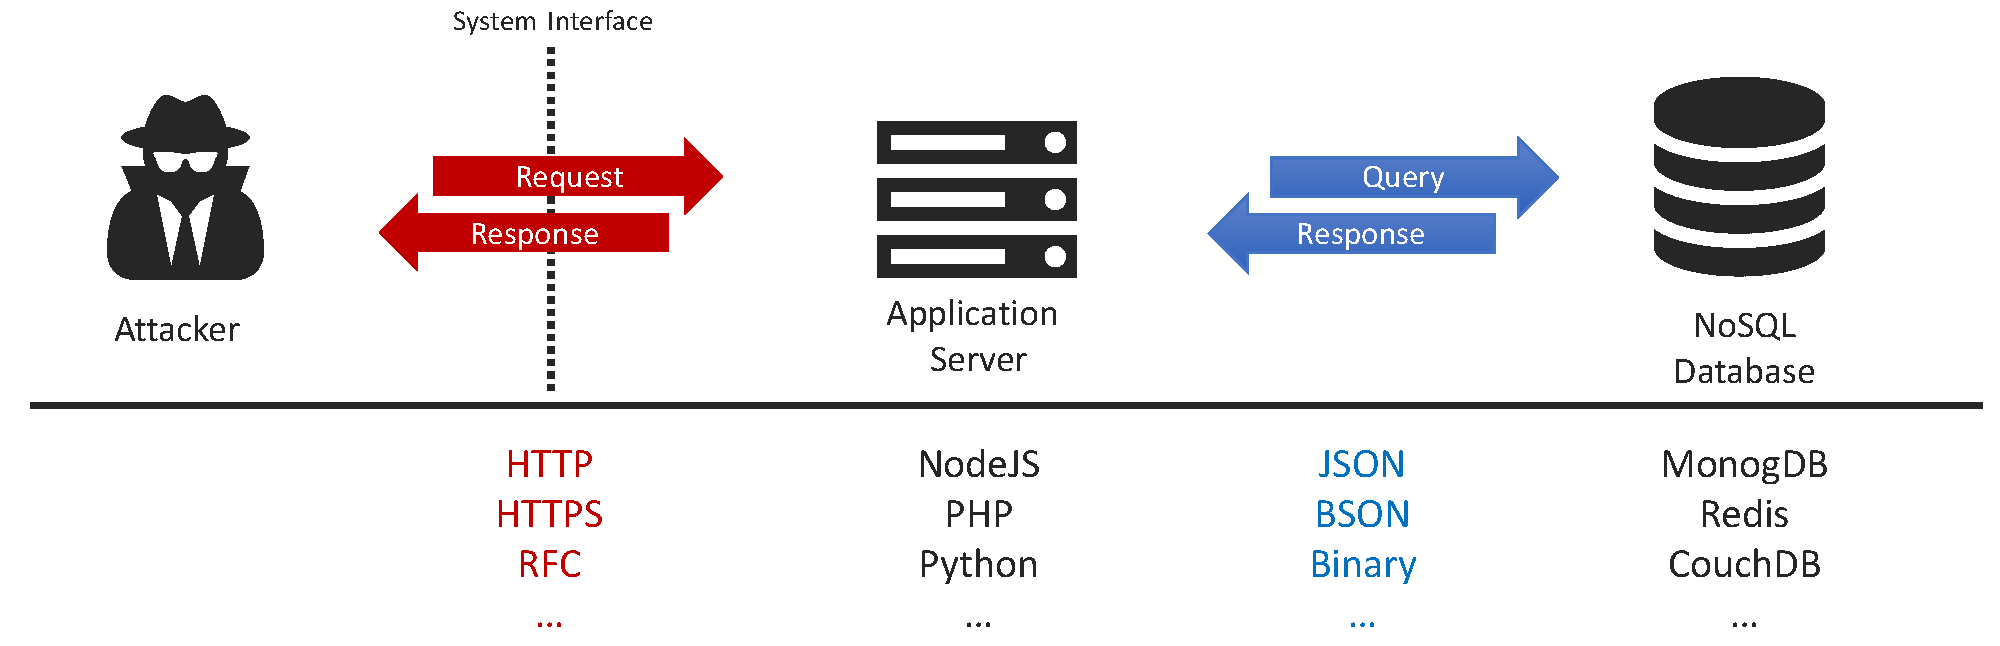
\includegraphics[width=1\linewidth]{Images/attacker_model_normal}
  \caption{Common attacker model for NoSQL injection}
  \label{fig:normalAttackerModel}
\end{figure}

% Objective

\subsection{Extended Attacker Model}

\begin{figure}[h]
\centering
  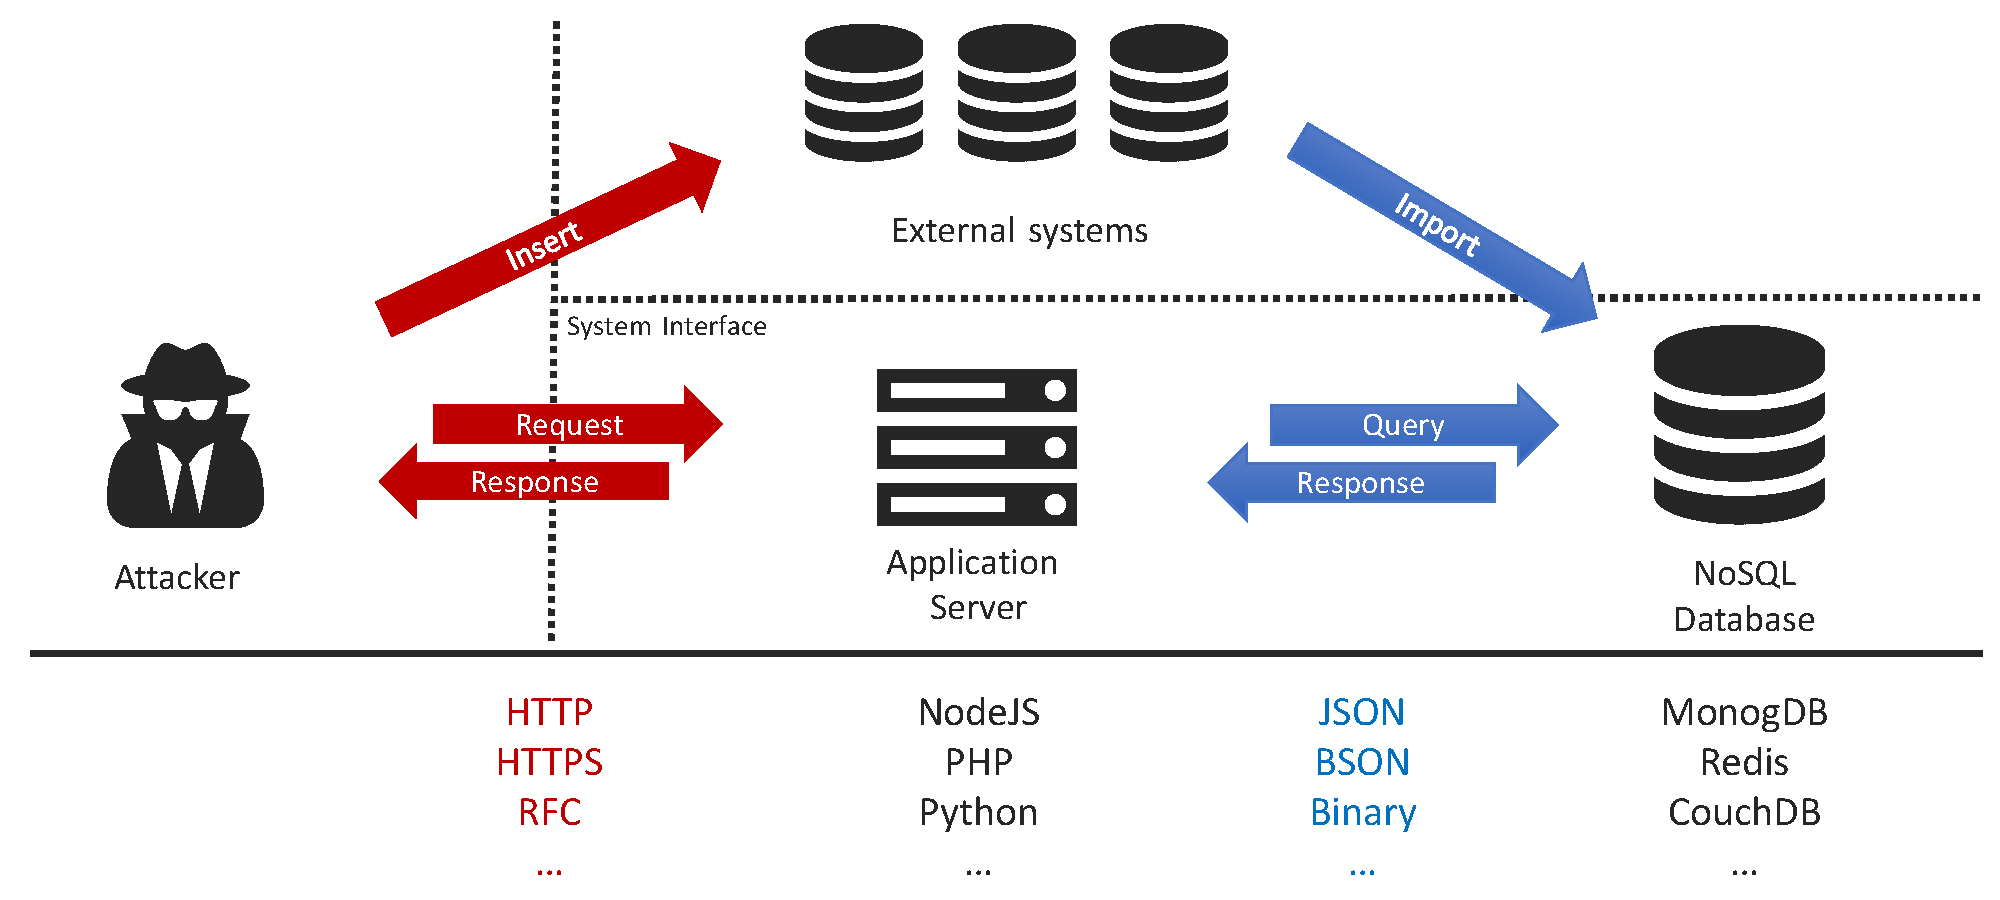
\includegraphics[width=1\linewidth]{Images/attacker_model_extended}
  \caption{Extended attacker model for NoSQL injection}
  \label{fig:extendedAttackerModel}
\end{figure}

% Objective

\subsection{Direct Attacker Model}

\begin{figure}[h]
\centering
  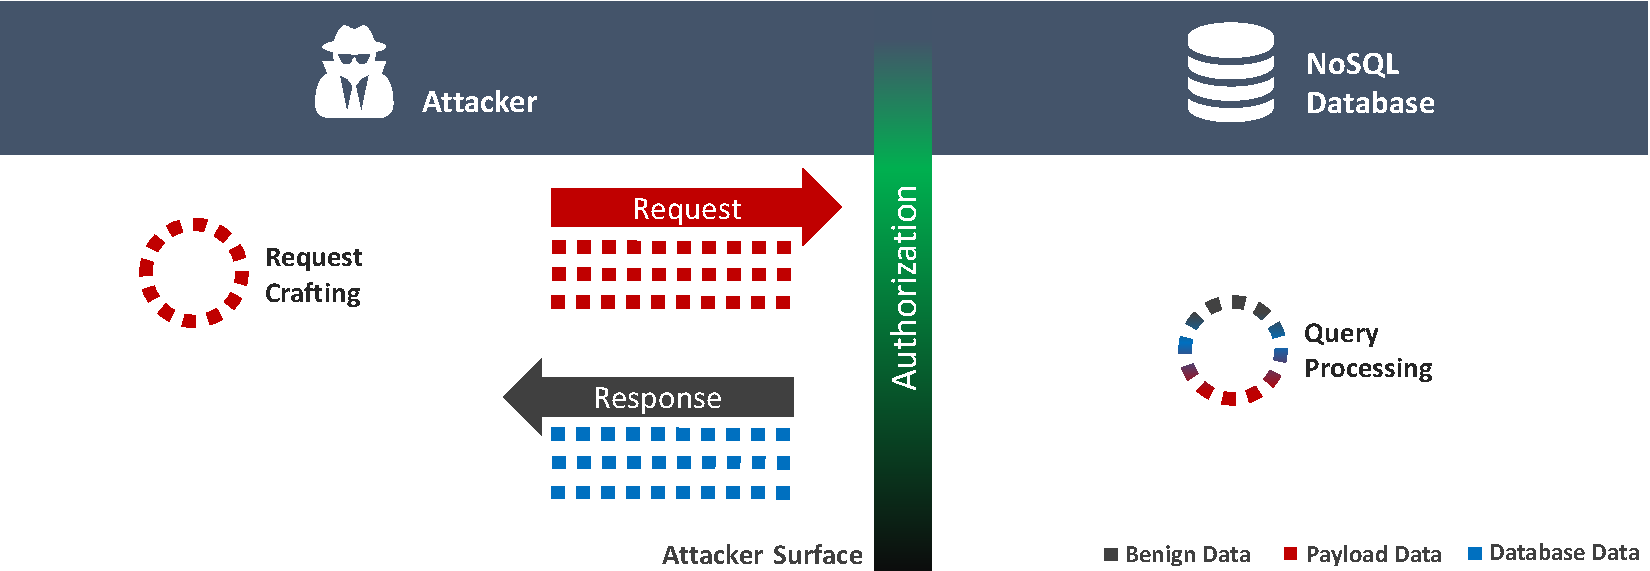
\includegraphics[width=1\linewidth]{Images/attacker_model_direct}
  \caption{Direct attacker model for NoSQL injection}
  \label{fig:extendedAttackerModel}
\end{figure}

% Objective


\section{Considered Technology Stack}
\subsection{Selected Databases}
\subsection{Selected Application Platforms}